\chapter{Backend} \label{chap:backend}

%Two basic transfer functions are shown in \cref{fig:methods:transfer_functions}.

%\begin{figure}[H]
%  \centering
%  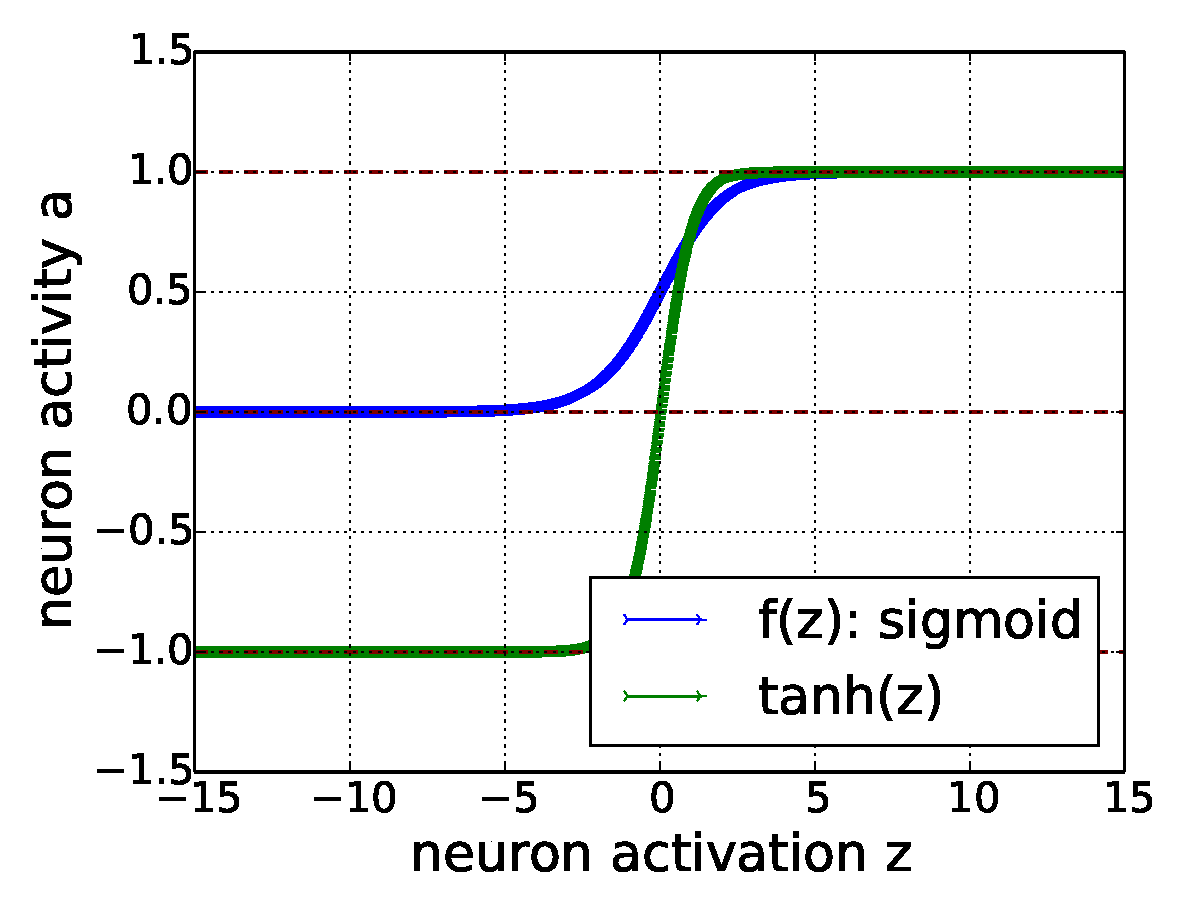
\includegraphics[width=0.7\textwidth]{transfer_functions.eps}
%  \caption{Transfer functions: \textit{Sigmoid} and \textit{Tanh}}
%  \label{fig:methods:transfer_functions}
%\end{figure}

For backend is developed own engine that runs on Raspberry Pi 3. The whole engine is coded in python, and aim practices wrote below.
\begin{itemize}
	\item Simplicity: Write straightforward code that is easily understandable for later rewriting.
	\item Modifiable: Write independent modules that can connect to others.
	\item Modularity: Write simple parts connected by clean interfaces
	\item Robustness: Robustness is the child of modularity and simplicity
\end{itemize}
%https://www.pharmasug.org/proceedings/2011/TT/PharmaSUG-2011-TT05.pdf


\section{Diagram description} \label{section:diagram description}

This section will briefly describe the architecture of the engine that is figured on a diagram - see  \cref{fig:vh_project_design}.

\begin{figure}[H]
  \centering
  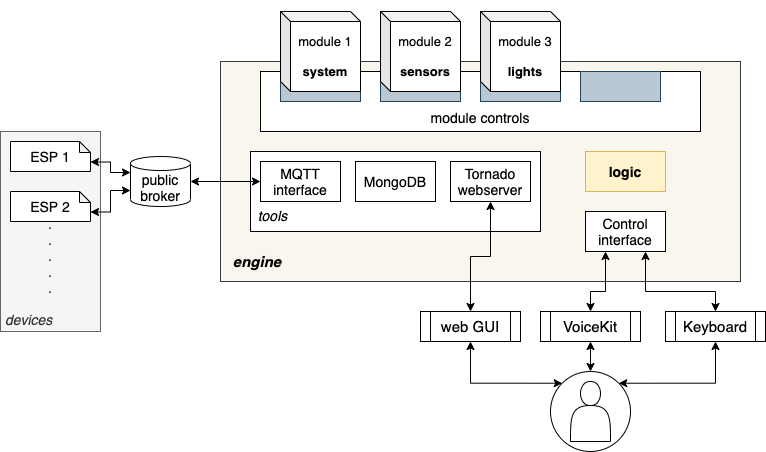
\includegraphics[width=0.85\textwidth]{img/vh_project_design.png}
  \caption{Project architecture}
  \label{fig:vh_project_design}
\end{figure}

Engine use tools like MQTT\footnote{\textbf{M}essage \textbf{Q}ueuing \textbf{T}elemetry \textbf{T}ransport}, MongoDB, Tornado web server that will be described later. Each of them runs in its thread and concurrently. These tools create a basis for modules and mediate main functionalities such as database, web server and communication. 


The engine is designed to easily remove, add or update any modules mutually independent that define functions used by a user interface. Each module will be described in the \cref{chap:modules}.

The engine also contains a separate block for logic. This block captures a command from the Voice Kit or keyboard interface, then browsing a predefined list of each module's commands and determines the best match for the user voice command or command written on the keyboard.

\section{Database} \label{section:database}

An auxiliary database is needed to store all the sensors data. For this purpose, it is used MongoDB due to the following advantages. 

MongoDB \citep{mongoDB_jayaram_2020} is an open-source document database build upon a NoSQL database and written in C++. Database's horizontal, scale-out architecture can support vast volumes of both data and traffic. One document can have others embedded in itself, and there is no need to declare the structure of documents to the system - documents are self-describing. 

Before using this type of database, we have to be familiar with different terminology instead of traditional SQL databases.
\begin{table}[H]
	\centering
	\begin{tabular}{|l|l|} \hline
		SQL Server & MongoDB \\ \hline
		Database & Database \\ \hline
		Table & Collection \\ \hline
		Index & Index \\ \hline
		Row & Document \\ \hline
		Column & Field \\ \hline
		Joining & Linking \& Embedding \\ \hline
		Partition & Sharding (Range Partition) \\ \hline
		Replication & ReplSet\\ \hline
	\end{tabular}
	\caption{MongoDB terminology}
	\label{tab:mongoDB_terminology}
\end{table}
%https://dzone.com/articles/why-mongodb

We use this type of database because it is famous for its use in agile methodologies, and the project tends to enlarge in the future. The main benefits are:
\begin{itemize}
	\item Document Oriented
	\item High availability - replication
	\item High scalability - sharding
	\item Dynamic - no rigid schema
	\item Flexible - field addition/deletion have less or no impact on the application
	\item Data representation in JSON\footnote{\textbf{J}ava\textbf{S}cript \textbf{O}bject \textbf{N}otation} or BSON\footnote{\textbf{B}inary \textbf{JSON}}
	\item Document-based query language that is nearly as powerful as SQL
\end{itemize}

For adding a new field, the field can be created without affecting all other documents in the collection, without updating a central system catalog, and without taking the system offline. 

In the project, we save all incoming messages from MQTT to MongoDB to a collection based on a name of interest module.

\section{Communication}

The backbone of the whole project is communication between a variety range of devices over the internet. Therefore had to been found robust, scalable and cost-effective protocols that will transmit messages and data securely. Based on the survey was chosen three protocols that, in combination, satisfy all our requirements, and we will delve deeper into them in the following sections.

\subsection{MQTT}

MQTT \citep{mqtt_malý_2016} is a standardized protocol by the OASIS MQTT Technical Committee used for message and data exchange. The protocol is designed specifically for the Internet of Things. The protocol is developed in vast language diversity from low-level to high-level programming language and designed at light versions for low-performance devices. Hence, it suits our use-case perfectly because each module possesses tons of various devices with limited resources that are already included or will arise later on.

\begin{figure}[H]
	\centering
	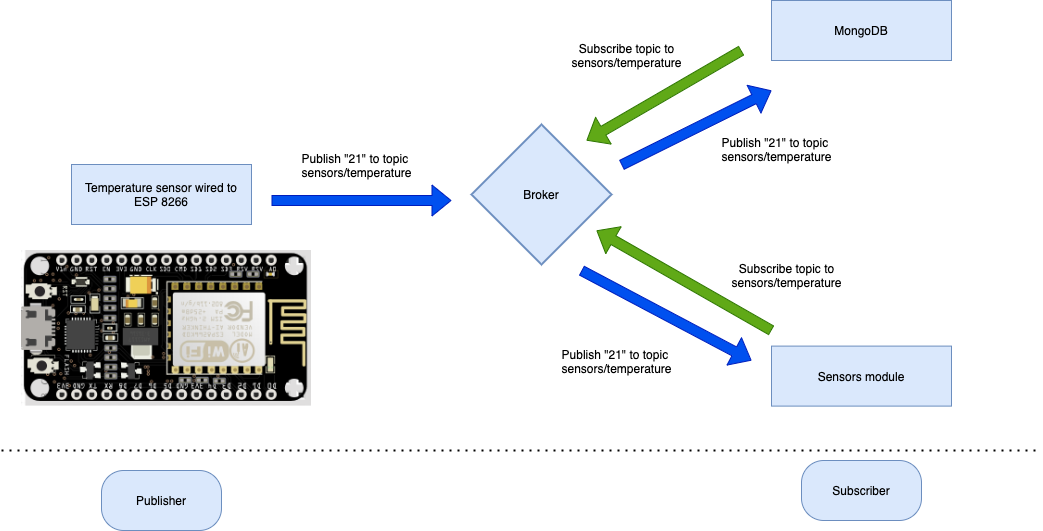
\includegraphics[width=0.85\textwidth]{img/MQTT_pub_sub_pattern.png}
	\caption{MQTT pub/sub pattern}
	\label{fig:MQTT_pub_sub_pattern}
  \end{figure}

The design principles are to minimize network bandwidth and device resource requirements whilst also attempting to ensure reliability and some degree of assurance of delivery. The protocol check errors by TCP and orchestrate communication by the central point - broker. The protocol architecture uses a publish/subscribe pattern (also known as pub/sub) shown in \cref{fig:MQTT_pub_sub_pattern}, which provides an alternative to traditional client-server architecture. Architecture decouples publishers and subscribers who never contact each other directly and are not even aware that the other exists. The decoupling giving us the following advantage:

\begin{itemize}
	\item Space decoupling: Publisher and subscriber do not need to know each other.
	\item Time decoupling: Publisher and subscriber do not need to run at the same time.
	\item Synchronization decoupling: Operations on both components do not need to be interrupted during publishing or receiving.
\end{itemize}

So, after some publisher publishes his message, it is handled by the broker who filters all incoming messages and distributes them to accredited subscribers. Filtering can base on topic or subject, content and type.

In our MQTT case, the messages are subject-based filtering, which means the filtering is based on a subject or topic and is part of each message. The client subscribes to the topics he is interested in, and the broker distributes the messages accordingly as shown in \cref{fig:MQTT_pub_sub_communication_diagram}.

\begin{figure}[H]
	\centering
	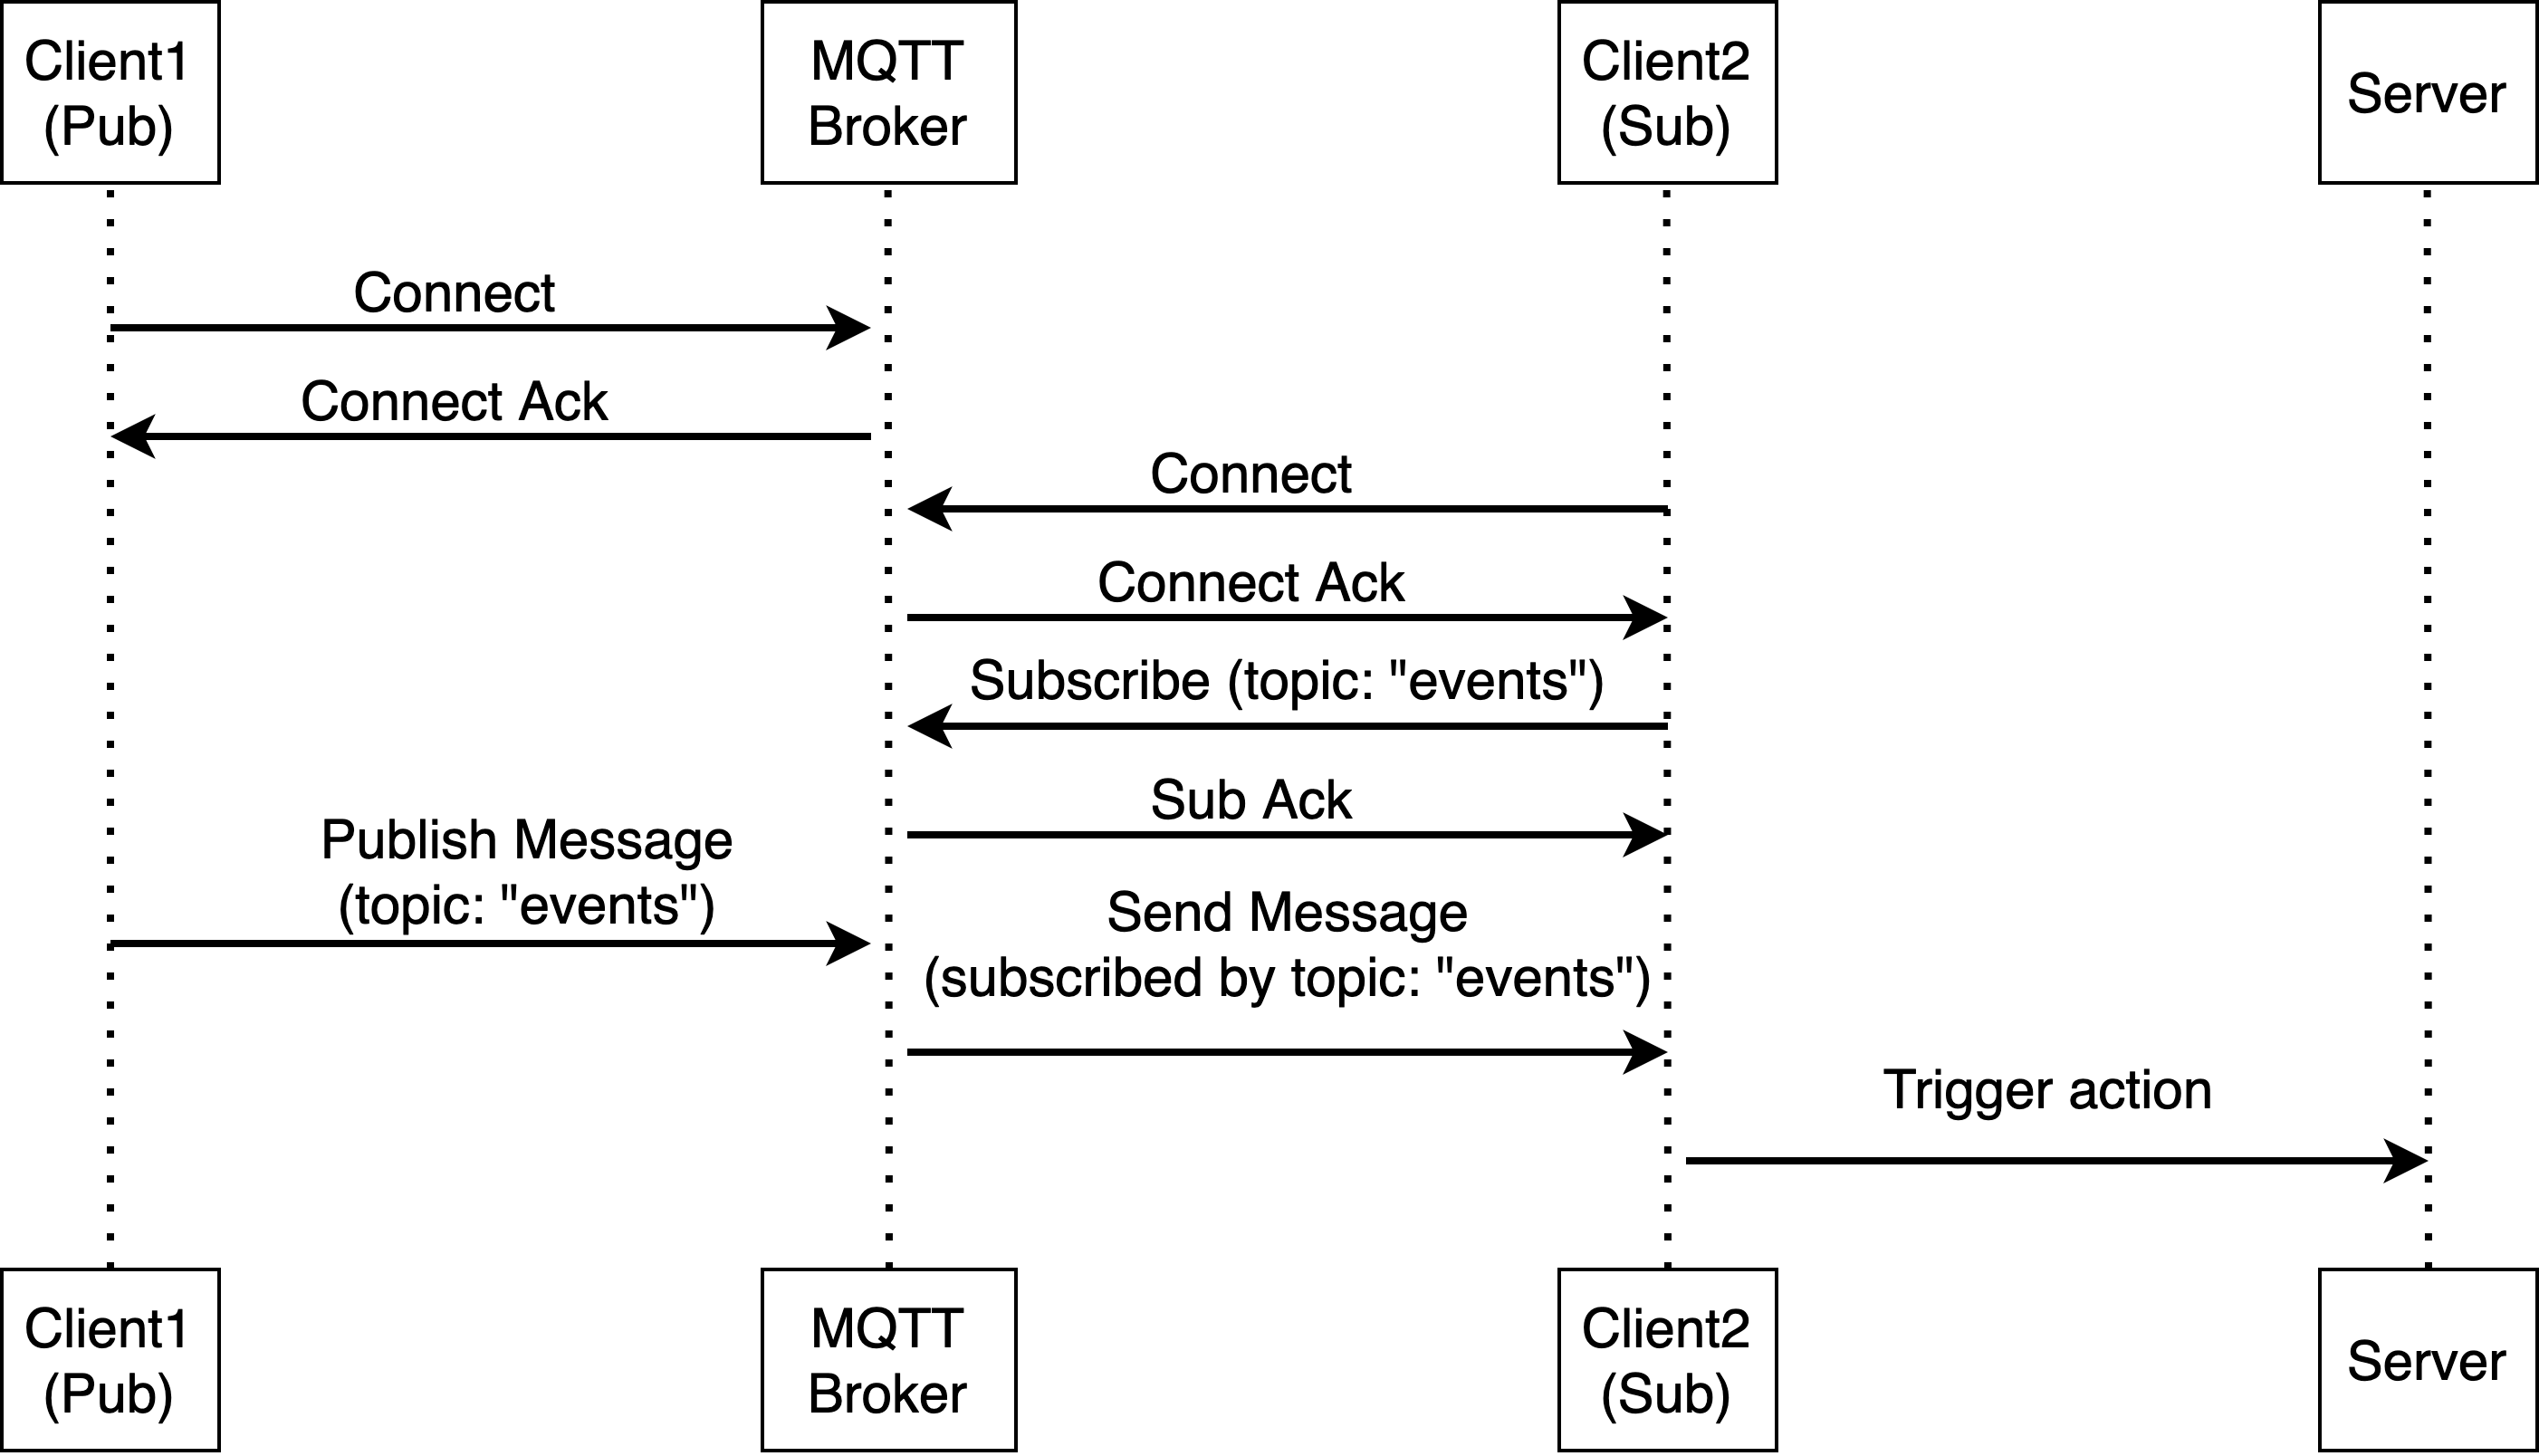
\includegraphics[width=0.85\textwidth]{img/MQTT_pub_sub_communication_diagram.png}
	\caption{MQTT pub/sub communication diagram}
	\label{fig:MQTT_pub_sub_communication_diagram}
  \end{figure}

The topics are generally strings with a hierarchical structure that allow different subscription levels. It is feasible to use wildcards to subscribe, for example, sensors/\# to receive all messages related to the sensors, such as sensors/temperature or sensors/illuminance.

The MQTT protocol has the Quality of Service (QoS) levels essential to any communication protocol.  The level of QoS can be specified for each message or topic separately according to its importance.

In MQTT, there are 3 QoS levels:

\begin{itemize}
	\item QoS 0: This level is often called "fire and forget" when a message is not stored and retransmitted by a sender.
	\item QoS 1: Is is guarantees that a message is delivered at least one time to the receiver. The message is stored on a sender until it gets a PUBACK packet from a receiver.
	\item QoS 2: It is the highest level, and it guarantees that each message received only once by the intended recipients.
\end{itemize}

It is vital to mention MQTT have the feature retained messages that are mechanisms where the broker stores the last retained message for a specific topic. This feature allows a client does not have to wait until a new message is published to know the last known status of other devices.
 
\subsection{WebSocket}
 
Now, all we need is communication between the client and the engine. WebSocket \citep{websocket_wang_salim_moskovits_2013} provides a low-latency, persistent, full-duplex connection between a client and server over TCP. The protocol is chiefly used for a real-time web application because it is faster than HTTP\footnote{\textbf{H}yper\textbf{t}ext \textbf{T}ransfer \textbf{P}rotocol} concerning more transfers by one connection. The protocol belongs to the stateful type of protocols, which means the connection between client and server will keep alive until either client or web server terminate it. The protocol fits for us in use between client and web server in case of real-time response.

The main benefits are:

\begin{itemize}
	\item Persistent - After an initial HTTP handshake, the connection keeps alive using a ping-pong process, in which the server continuously pings the client for a response. It is a more efficient way than establishing and terminating the connection for each client request and server response. Server terminating connection after an explicit request from the client, or implicitly when the client goes offline.
	\item Secure - WebSocket Secure uses standard SSL and TLS encryption to establish a secure connection. Although we do not pursue this issue in our work, it is a valuable feature to add later.
	\item Extensible - Protocol is designed to enabling the implementation of subprotocols and extensions of additional functionality such as MQTT, WAMP, XMPP\footnote{E\textbf{x}tensible \textbf{M}essaging and \textbf{P}resence \textbf{P}rotocol}, AMQP\footnote{\textbf{A}dvanced \textbf{M}essage \textbf{Q}ueuing \textbf{P}rotocol }, multiplexing and data compression. This benefit makes WebSockets a future-proof solution for the possible addition of other functionalities.
	\item Low-latency - WebSocket significantly reduces each message's data size, drastically decreasing latency by eliminating the need for a new connection with every request and the fact that after the initial handshake, all subsequent messages include only relevant information.
	\item Bidirectional - This enables the engine to send real-time updates asynchronously, without requiring the client to submit a request each time, as is the case with HTTP. 
\end{itemize}

We will apply this protocol for transfer between clients such as Voice Kit, keyboard or web interface and engine in case of real-time response.

\subsection{REST}

In other cases like fetching data only once or data that is not required very frequently, we use RESTfull\footnote{\textbf{R}\textbf{E}presentational \textbf{S}tate \textbf{T}ransfer} web service on a web server. This service enables us to transfer a lightweight data-interchange format JSON trivially and reliably - see \cref{fig:REST_schema}. We use a standard GET REST request on a defined URI and then decode it like JSON for fetching data.

\begin{figure}[H]
  \centering
  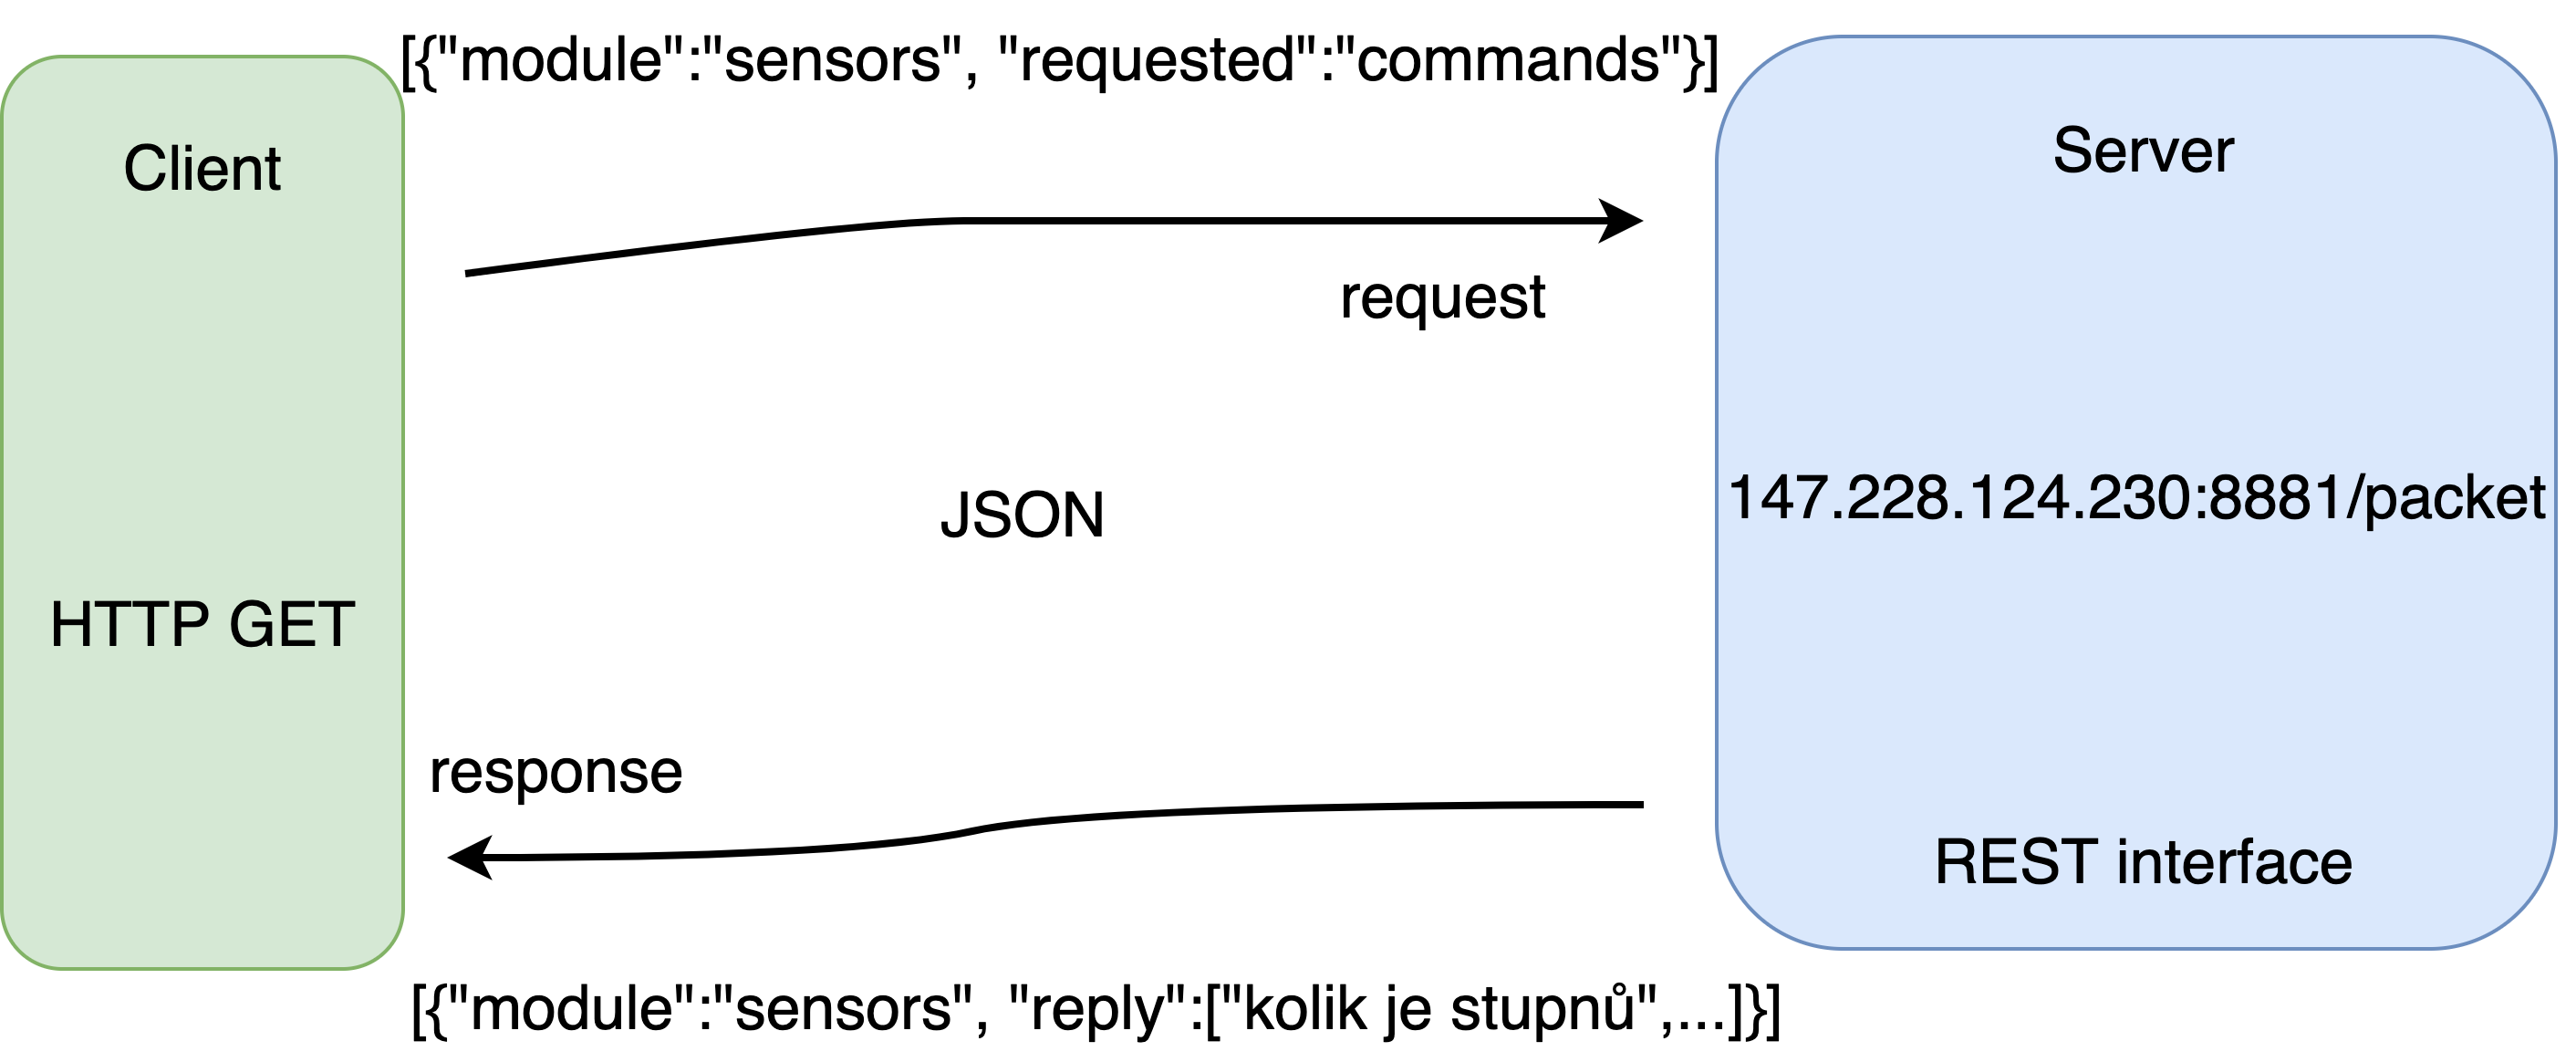
\includegraphics[width=0.85\textwidth]{img/REST_schema.png}
  \caption{REST principle}
  \label{fig:REST_schema}
\end{figure}

\section{Controllers}

\subsection{Keyboard}

The keyboard is a python script with a particular purpose for developing new voice commands. This script opens up a CLI\footnote{\textbf{c}ommand-\textbf{l}ine \textbf{i}nterface} built upon a voicehome controller. Over the command-line can be easily typed a voice command with high accuracy, thus fully debugged in various forms.

\subsection{Voice Kit}

Voice kit \citep{aiy_projects} is a building kit made by google that lets users create their natural language processor and connect it to the Google Assistant or Cloud Speech-to-Text service. By pressing a button on top, users can ask questions and issue voice commands to their programs. All of this fits in a handy little cardboard cube powered by a Raspberry Pi. 

\begin{figure}[H]
	\centering
	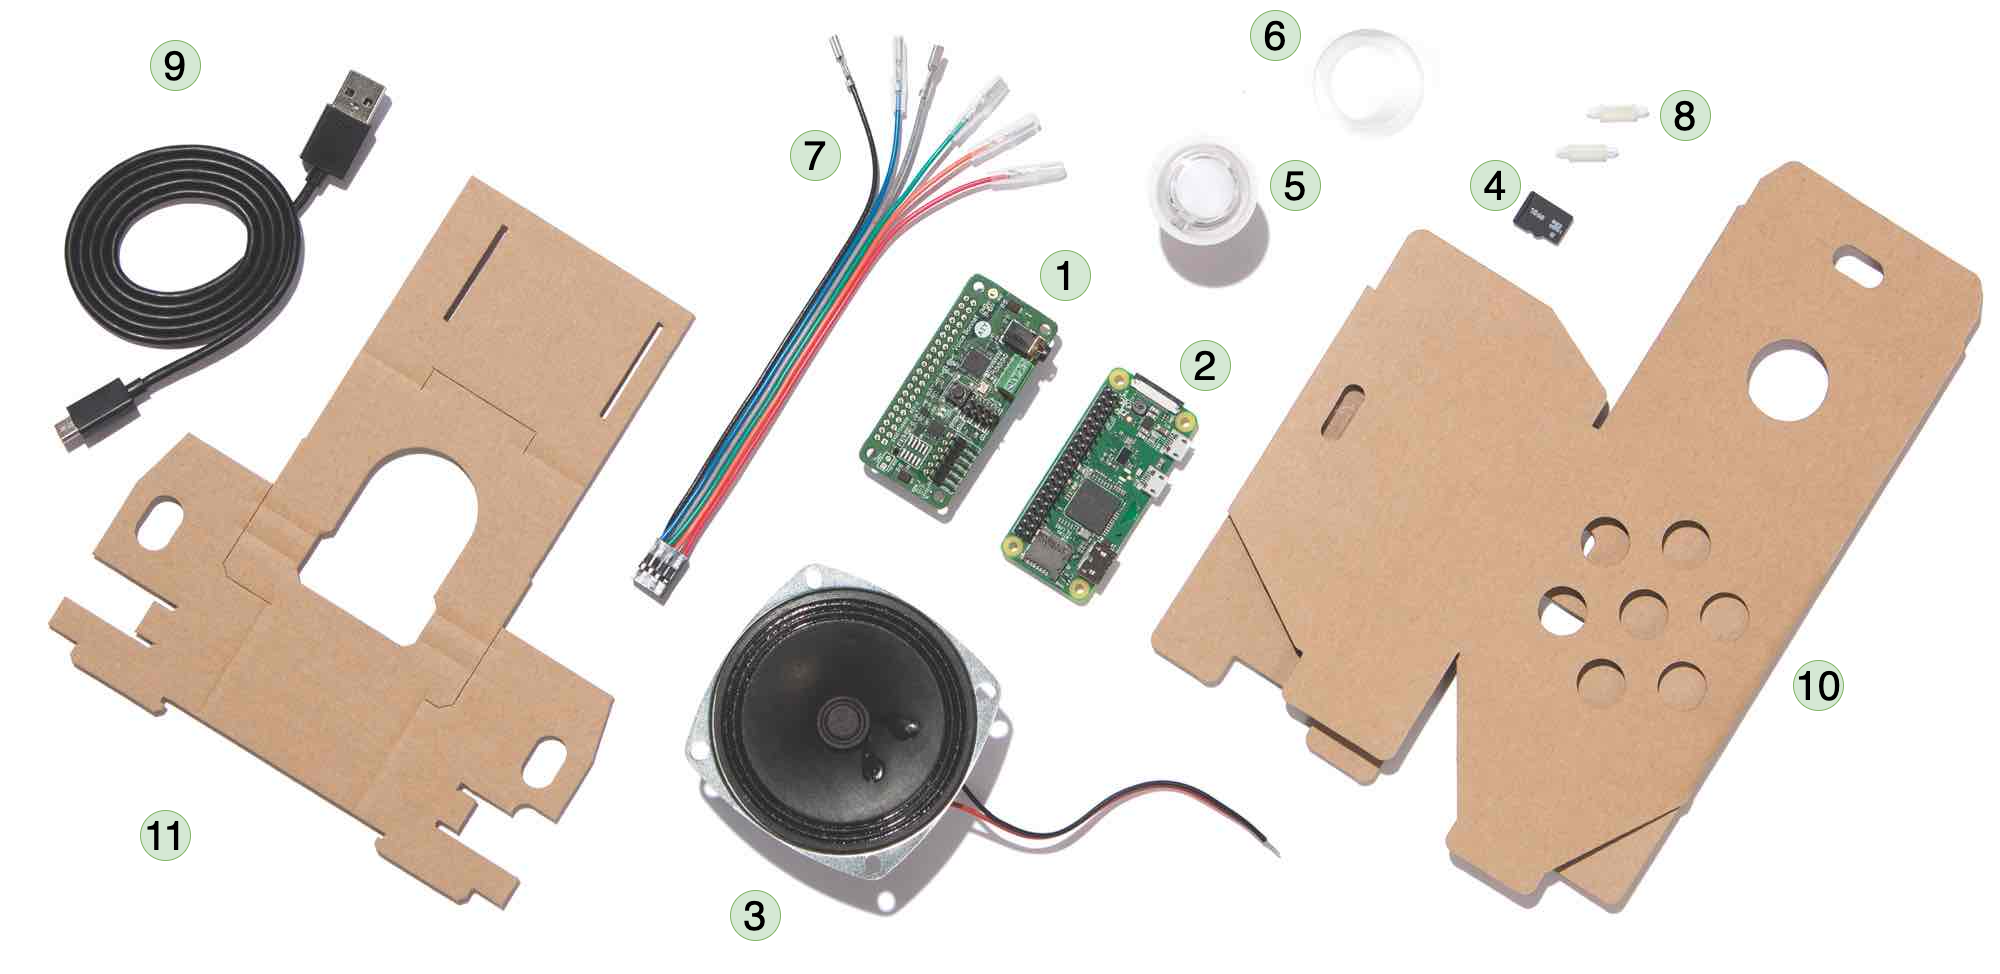
\includegraphics[width=0.85\textwidth]{img/voice_kit.png}
	\caption{Voice kit materials}
	\label{fig:voice_kit}
  \end{figure}

The user must assemble the cube himself from the following components showed in \cref{fig:voice_kit}:

\begin{enumerate}
	\item Voice bonnet
	\item Raspberry Pi Zero WH
	\item Speaker
	\item Micro SD card
	\item Push button
	\item Button nut
	\item Button harness
	\item Standoffs
	\item Micro USB cable
	\item Speaker box cardboard
	\item Internal frame cardboard
\end{enumerate}

In this project, we connected the Voice kit to the faculty Speechcloud from \cref{chap:dialog_systems}.

\subsection{Website}

As the second interface next to the already mentioned Voice Kit is a website. The server is coded in python with the tornado framework.

The website's architecture aims to use it via a portable device like a smartphone and tablet or touch screen attached to the wall. Therefore the website is constructed to be responsible, straightforward and touch-friendly. The website's use-cases are to able the user to monitor ESP, sensors, lights, weather and voice commands, display historical sensors data, feasible voice commands and description of them, trigger lights and modules.

To build up a web page are further used libraries and frameworks like Bootstrap, JQuery and Dygraphs, used to facilitate work and make the page more robust. Each of them is described in the sections below. Web site use for fetching data from engine already mentioned WebSocket and REST API. 